\section{Suffix Tries}

\begin{Definition}
  Let $S = \{S_0, S_1, \ldots, S_{N-1}\}$ be a set of strings over an alphabet $\Sigma$. A \defi{trie}{Trie} $\mathcal{T}$ is a tree, where each node represents a different prefix in the set $S$. The root represents the empty prefix $\varepsilon$. Vertex $u$ representing prefix $Y$ is a child of vertex $v$ representing prefix $X$, if and only if $Y = Xc$ for some character $c \in \Sigma$. The edge $(v,u)$ is then labeled $c$.\\
  If $S$ is the set of all suffixes of a string $T$, the trie is called \defi{suffix trie}{Suffix Trie} of $T$.
\end{Definition}

\begin{Example}
  Figure~\ref{fig:suffixTrieExample} shows the suffix trie for the string "banana\$". The dollar sign "\$" is a sentinel that does not appear elsewhere in the text (and is lexicographically smaller than all other symbols). This guarantees, that no suffix is a prefix of another suffix and the suffix trie therefore has $n+1$ leaves.
  \begin{figure}[htb]
    \centering
    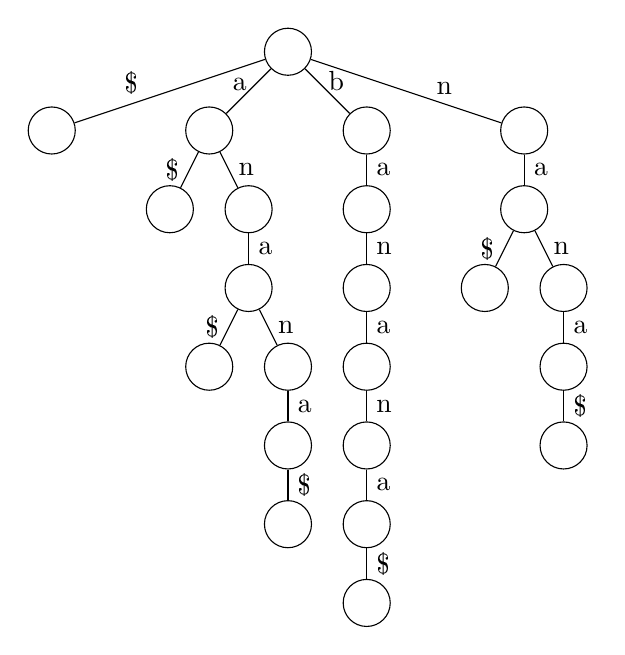
\begin{tikzpicture}
  \tikzstyle{vertex}=[circle,draw,minimum size=17pt,inner sep=0pt]
  \node[vertex] (epsilon) at (0,0) {};

  \node[vertex] (d) at (-3,-1) {};
  \draw (epsilon) -- (d) node[above,pos=0.7] {\$};

  \node[vertex] (a) at (-1,-1) {};
  \draw (epsilon) -- (a) node[above,pos=0.7] {a};

  \node[vertex] (ad) at (-1.5,-2) {};
  \draw (a) -- (ad) node[left,pos=0.5] {\$};

  \node[vertex] (an) at (-0.5,-2) {};
  \draw (a) -- (an) node[right,pos=0.5] {n};

  \node[vertex] (ana) at (-0.5,-3) {};
  \draw (an) -- (ana) node[right,pos=0.5] {a};

  \node[vertex] (anad) at (-1,-4) {};
  \draw (ana) -- (anad) node[left,pos=0.5] {\$};

  \node[vertex] (anan) at (0,-4) {};
  \draw (ana) -- (anan) node[right,pos=0.5] {n};

  \node[vertex] (anana) at (0,-5) {};
  \draw (anan) -- (anana) node[right,pos=0.5] {a};

  \node[vertex] (ananad) at (0,-6) {};
  \draw (anana) -- (ananad) node[right,pos=0.5] {\$};

  \node[vertex] (b) at (1,-1) {};
  \draw (epsilon) -- (b) node[above,pos=0.7] {b};

  \node[vertex] (n) at (3,-1) {};
  \draw (epsilon) -- (n) node[above,pos=0.7] {n};

  \node[vertex] (ba) at (1,-2) {};
  \draw (b) -- (ba) node[right, pos=0.5] {a};

  \node[vertex] (ban) at (1,-3) {};
  \draw (ba) -- (ban) node[right, pos=0.5] {n};

  \node[vertex] (bana) at (1,-4) {};
  \draw (ban) -- (bana) node[right, pos=0.5] {a};

  \node[vertex] (banan) at (1,-5) {};
  \draw (bana) -- (banan) node[right, pos=0.5] {n};

  \node[vertex] (banana) at (1,-6) {};
  \draw (banan) -- (banana) node[right, pos=0.5] {a};

  \node[vertex] (bananad) at (1,-7) {};
  \draw (banana) -- (bananad) node[right, pos=0.5] {\$};

  \node[vertex] (na) at (3,-2) {};
  \draw (n) -- (na) node[right,pos=0.5] {a};

  \node[vertex] (nad) at (2.5,-3) {};
  \draw (na) -- (nad) node[left,pos=0.5] {\$};

  \node[vertex] (nan) at (3.5,-3) {};
  \draw (na) -- (nan) node[right,pos=0.5] {n};

  \node[vertex] (nana) at (3.5,-4) {};
  \draw (nan) -- (nana) node[right,pos=0.5] {a};

  \node[vertex] (nanad) at (3.5,-5) {};
  \draw (nana) -- (nanad) node[right,pos=0.5] {\$};
\end{tikzpicture}

    \caption{The suffix trie for the string "banana\$".}
    \label{fig:suffixTrieExample}
  \end{figure}
\end{Example}

To construct a trie over string set $S = \{S_0, \ldots, S_{N-1}\}$, we need $\mathcal{O}(\vert S_0 \vert + \ldots + \vert S_{N-1} \vert)$ steps. This bound is tight: If all characters are pairwise distinct in all strings and no two strings share a character, than the number of different prefixes and therefore vertices is given by $1 + \sum_{i=0}^{N-1} \vert S_i \vert$, where the additional $1$ represents the empty prefix $\varepsilon$.\\
The time needed to search for a string $T$ of length $m = \vert T \vert$ in the trie depends on the implementation of the tree. If the children of each vertex are stored in a list, the time is in $\mathcal{O}(m\sigma)$. If the children are stored in a sorted array (using the order of the characters in the alphabet), the time is in $\mathcal{O}(m\log \sigma)$. By using a hash table and perfect hashing, the time is in $\mathcal{O}(m)$.

The space needed to store the suffix trie $\mathcal{T}$ for a string of length $n$ is in $\mathcal{O}{(n^2\log \sigma + n^2\log n)}$ bits. The first summand is the space needed to store the $\mathcal{O}(n^2)$ edge labels of one character $c \in \Sigma$ each. The second summand is the space needed to store the pointers to the children of each node.

